\section{Rendering} \label{sec:rendering}
Die Evaluation der Limesfläche erfolgt für die Unterteilungsalgorithmen Butterfly, Modified Butterfly und Loop mit Hilfe eines interpolierenden Renderers.
Die Evaluation der Limesfläche der Unterteilungsalgorithmen Catmull-Clark und Doo-Sabin hingegen mittels des GLU NURBS Interfaces.
Die Kontrollnetze dieser beiden Unterteilungsalgorithmen basieren auf nichtuniformen B-Splines.

\subsection{B-Spline}
Ein approximierender, oder interpolierender Spline ist eine stückweise aus Polynomen zusammengesetzte Funktion, die so konstruiert wird, dass sie die geforderten Eigenschaften, wie beispielsweise hinreichende Glätte oder Uniformität, erfüllt.

Um den Grad eines Splines zu beschränken und dennoch eine glatte Kurve durch beliebig viele Kontrollpunkte bestimmen zu können, muss die Auswirkung der einzelnen Basisfunktionen in natürlicher Weise begrenzen werden.
Isaac Jacob Schoenberg hat den Begriff B-Spline (für Basis-Spline) geprägt und über das Faltungsintegral motiviert, Carl de Boor hat 1978 die algorithmische und numerisch stabile Konstruktion der Basis geliefert.
Die auf diese Weise konstruierte Basis hat diverse Eigenschaften, die man auch bei subdivision surfaces benötigt. \cite{kroemker:2008}

B-Splines kommen hauptsächlich in der computergestützten Konstruktion \textit{CAD} und der computergestützten Fertigung \textit{CAM} zum Einsatz.

\begin{figure}[h]
  \centering
  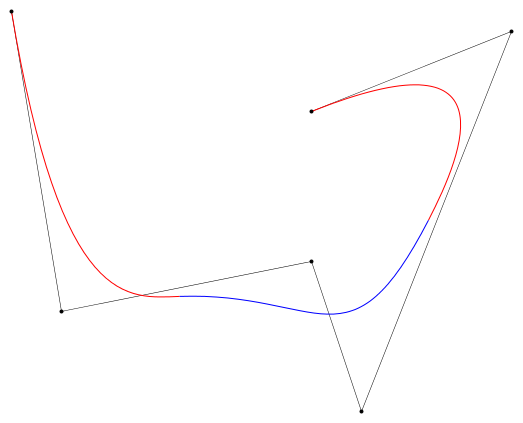
\includegraphics[width=0.7\textwidth]{content/media/b-spline_curve.png}
  \caption{B-Spline Kurve \cite{b-spline:2016}}
  \label{fig:b-spline}
\end{figure}

\subsubsection{Definition}
Definiert werden B-Splines folgendermaßen:

Für einen gegebenen Knotenvektor aus $m + 1$ aufsteigend sortierten Werten $t_{i} \in [0, 1]$ des Einheitsintervalls

\begin{align*}
0 \leq t_{0} \leq t_{1} \leq \dots \leq t_{m} \leq 1
\end{align*}

ist ein B-Spline vom Grad n eine parametrisierte Kurve

\begin{align*}
f: [t_{n}, t_{m-n}[ \hspace{5mm} \to \hspace{5mm} \mathbb{R}^{2}
\end{align*}

\begin{align*}
t \hspace{5mm} \mapsto \hspace{5mm} \sum_{i=0}^{m-n-1} b_{i,n}(t)P_{i}
\end{align*}

mit $m - n$ Kontrollpunkten $\{P_{0}, \dots , P_{m-n-1}\}$ und rekursiv definierten Basispolynomen

\begin{align*}
b_{j, 0}(t) := 
\begin{cases}
1 \hspace{2mm} $für$ \hspace{2mm} t_{j} \leq t < t_{j+1}\\
0 \hspace{2mm} sonst\\
\end{cases}
\end{align*}

\begin{align*}
b_{j, n}(t) := \frac{t - t_{j}}{t_{j + n} - t_{j}} b_{j, n-1} (t) + \frac{t_{j + n + 1} - t}{t_{j + n + 1} - t_{j + 1}} b_{j + 1, n - 1} (t).
\end{align*}

Für identische Knoten $t_{j} \equiv t_{j + 1}$ wird $b_{j, 0} (t) \equiv 0$ und es reduziert sich $b_{j, 1}$ zu

\begin{align*}
b_{j, 1}(t) := \frac{t_{j + 2} - t}{t_{j + 2} - t_{j + 1}} b_{j + 1, 0} (t).
\end{align*}

\cite{kroemker:2008}

Im Gegensatz zu Bezierkurven kann der Grad vorgeschrieben werden und beliebig viele Kontrollpunkte entlang des Splines definiert werden.
Dafür muss lediglich ein Kontrollvektor zur Verfügung gestellt werden, der die Summe aus gefordertem Grad und Anzahl an Kontrollpunkten um mindestens eins übersteigt.
Zudem ist der B-Spline nicht auf dem gesamten Intervall definiert $[t_{0}, t_{m}[$, sondern nur auf $[t_{n}, t_{m - n}[$. \cite{kroemker:2008}

B-Splines werden als uniform bezeichnet, wenn die Knoten das Intervall zur Parametrisierung der Kurve äquidistant unterteilen.
Andernfalls werden sie als nichtuniform bezeichnet. \cite{kroemker:2008}

Ein offen uniformer B-Spline wiederholt den ersten und letzten Knoten der Gradzahl entsprechend $(n + 1)$ mal, um den Spline bis an diese Punkte heranzuführen.
Ein solcher offen uniformer B-Spline, dessen Anzahl an Kontrollpunkten den Grad genau um genau eins übersteigt, entspricht einem Bézier-Spline. \cite{kroemker:2008}

Eine wichtige Eigenschaft von B-Splines ist ihre \textit{Verfeinerbarkeit}.
Dabei können neue Kontrollpunkte so eingefügt werden, dass sich die durch den B-Spline beschriebene Kurve nicht ändert.
Die Verfeinerungsgleichung lautet folgendermaßen:

\begin{align*}
B_{n} (t) = \frac{1}{2^{n}} \sum_{k=0}^{n + 1} \left(
\begin{array}{c}
n + 1\\
k
\end{array}
\right) B_{n}(2t - k).
\end{align*}

\cite{kroemker:2008}
